THz Spectroscopy performed in the time domain also known as THz Time-Domain Spectroscopy (THz-TDS) is a spectroscopy technique which commonly is based on the optical excitation of photoconductive antennas. This type of THz spectroscopy was made possible through the development of the femtosecond laser since the photoconductive antennas (PCA) require ultrafast laser pulses for the generation of broadband THz radiation. A more elaborate description of the generation and detection mechanisms is presented in sections \ref{sec:thz-generation} and \ref{sec:thz-detection}. Additionally, compared to other spectroscopy methods such as Fourier-transform spectroscopy which only measures the power spectrum, THz-TDS has the advantage that both the amplitude and phase of the radiation can be measured. Another property of THz-TDS is that the radiation employed is non-ionizing which makes it safer to use without additional security protocols as for example in case of x-rays. In addition, a wide range of materials are transparent in the THz energy range so that underlying layers can be probed without physically altering the sample. Finally, an important aspect of THz-TDS especially in the context of this work is that it can be used for the characterization of THz devices such as waveguides, photonic crystals and metamaterials \cite{Horlick68, Jepsen2011}.
% add that it's useful in our case, for device characterization. Jepsen (done)

\section{Generation of THz radiation}
\label{sec:thz-generation}
There exists several techniques based on different mechanisms which can be employed in the TDS setups for the generation of THz radiation \cite{Jepsen2011}. Specifically, in this work we use PCAs for this purpose. As mentioned earlier in this case a femtosecond laser is used to generate a train of ultrashort laser pulses with bandwidths in the THz range. The laser pulses triggers the PCA which in turn emmits radiation with a similar bandwidth as the laser pulses. In the following additional details about this process will be presented.
Figure \ref{fig:PCA} shows a sketch of a PCA and its main components. The PCA consists of a semiconductor substrate with a hemispherical lens attached to the surface. On the opposing surface a photoconductive layer is added on which a conducting antenna structure is applied using photolithography. Specifically, the antenna structure consists of two parts or electrodes separated by a photoconductive gap, across this gap a bias voltage is applied. This means that when incoming laser pulses with sufficient photon energy illuminate the gap electrons in the semiconductor are excited into the conduction band which in turn allows a photocurrent to flow between the electrodes driven by the bias potential difference. 

\begin{figure}[H]
    \centering
    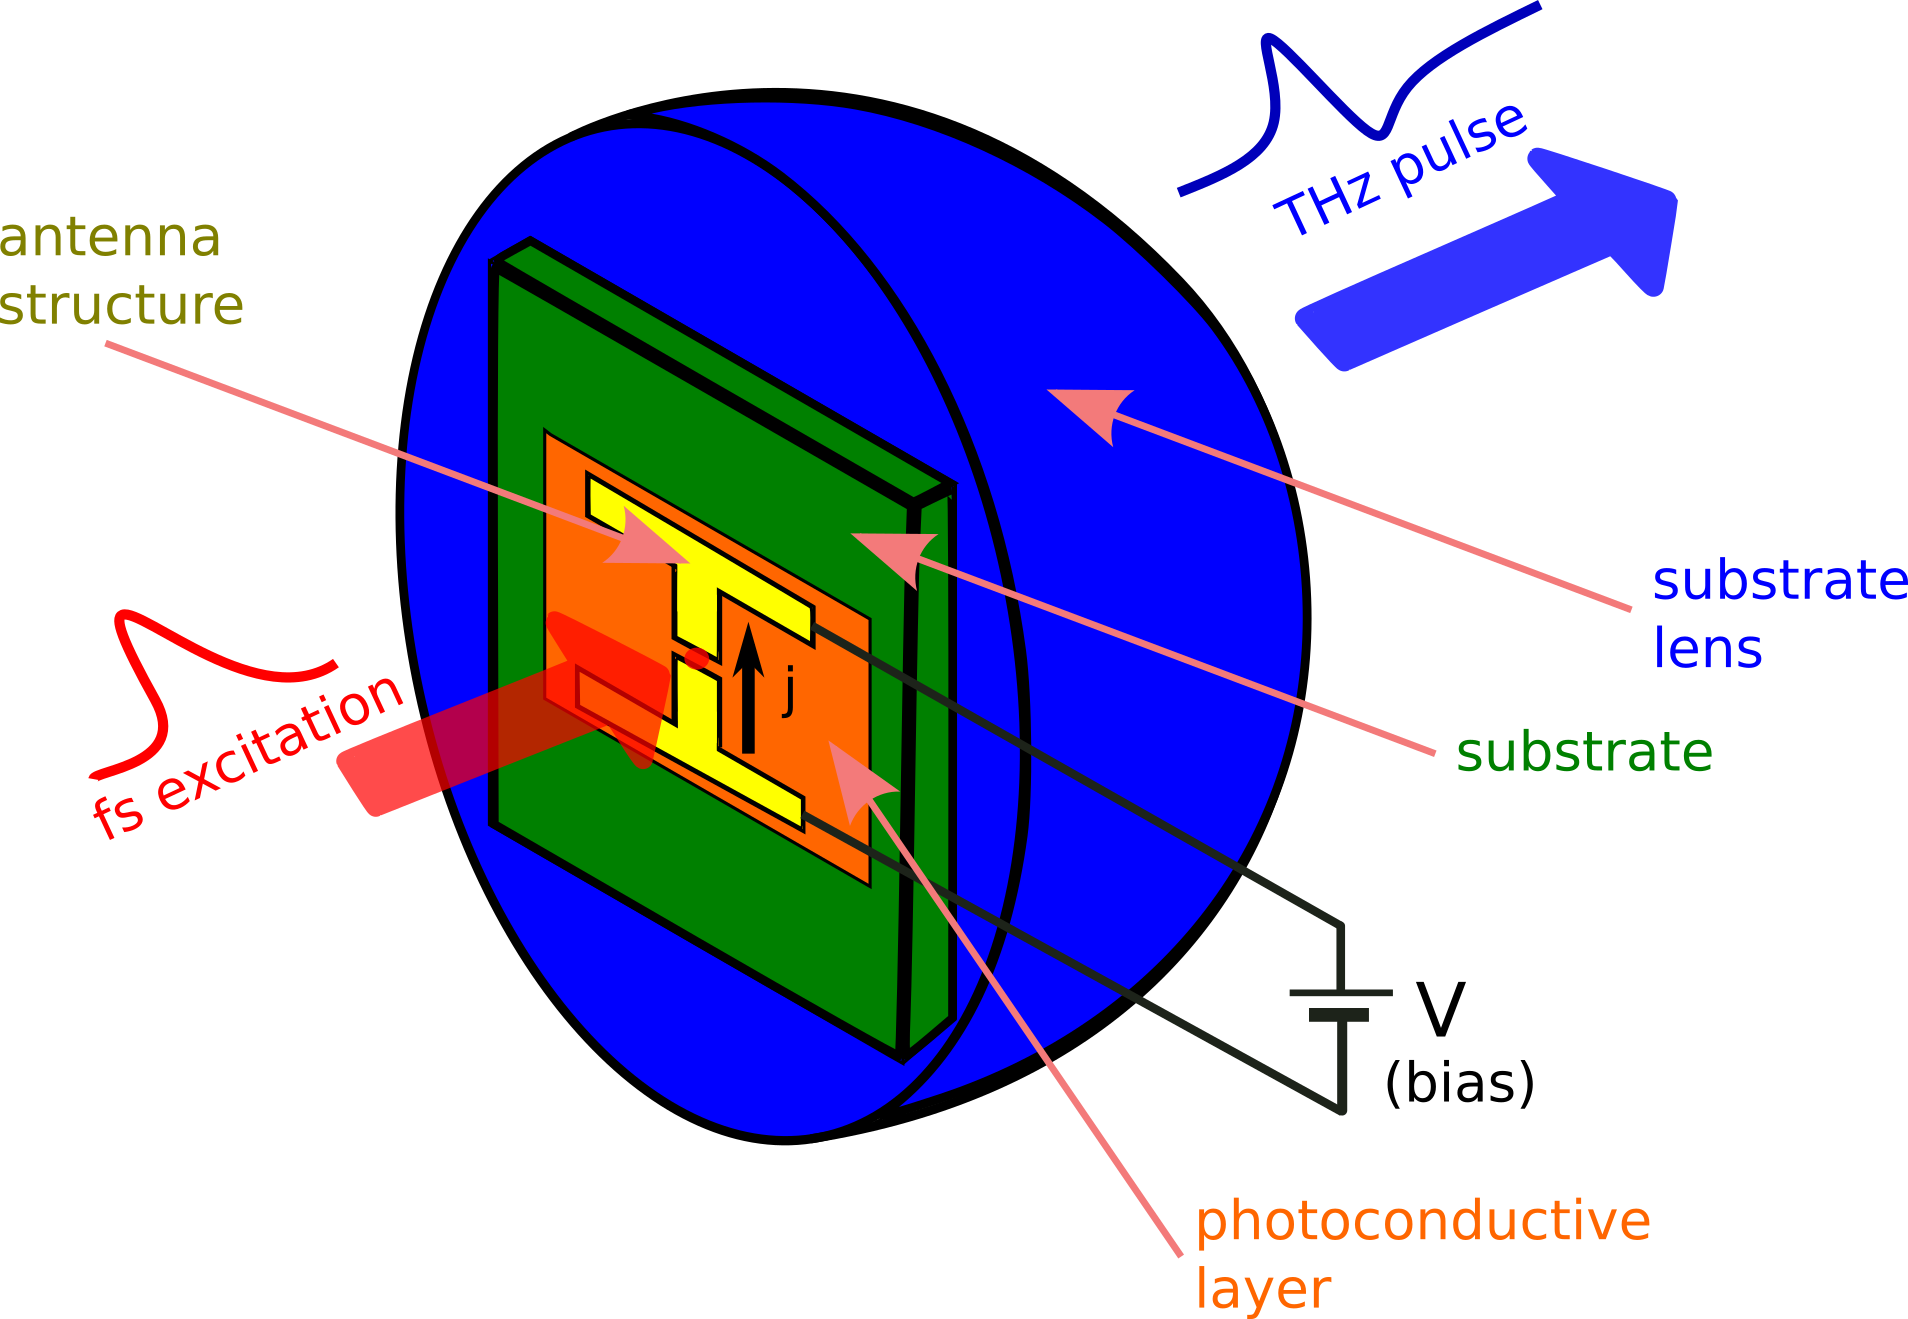
\includegraphics[scale=0.5]{images/TDS/PCA.png}
    \caption{Example of a PCA used for THz generation. The incoming laser pulse generates free charge carriers in the semiconductor substrate. The free charge carriers move due to the applied voltage so that a current flows between the anode and cathode. This high acceleration of the charge carriers causes them to emit radiation in the THz range. The shape of the silicon lens(shown in blue) prevents total internal reflection due to the high impedance difference.}
    \label{fig:PCA}
\end{figure}

The Drude-Lorentz model allows us to model the motion of the charge carriers which we assume to be predominantly consisting of electrons since they have a lower effective mass and therefore also a lower inertia compared to the holes. With this the photocurrent $j(t) = -e n(t) v(t)$ can be described via a coupled set of rate equations as follows:
\begin{equation}
    \frac{dn}{dt} = - \frac{n}{\tau_c} + G(t)
\end{equation}
\begin{equation}
    \label{eq:photocurrent_2}
    \frac{dv}{dt} = - \frac{v}{\tau_s} + \frac{e}{m^*}\left(E_0 - \frac{P_{sc}(t)}{\eta \epsilon} \right)
\end{equation}
\begin{equation}
    \frac{dP_{sc}(t)}{dt} = -\frac{P_{sc}(t)}{\tau_r}+j(t)
\end{equation}
where $n(t)$, $v(t)$, $e$ and $m^*$ denotes the density, velocity, charge and effective mass of the electrons respectively. $G(t)$ describes the increase of electron density in the illuminated area which therefore scales with the intensity of the laser pulse $I_L$. Additionally, due to the concurrent generation of holes and subsequent separation from the electrons an electric polarization $P_{sc}(t)$ is formed. This polarization field screens the local bias field $E_0$ where the screening strength is corrected by the effective permittivity $\epsilon$ of the semicondutor and the factor $\eta$, hence the correctional term to the field strength $E_0$ in equation \ref{eq:photocurrent_2}. The three times $\tau_c$, $\tau_s$ and $\tau_r$ serve as dampening factors and model different rate-lowering phyiscal processes which therefore depend on the semiconductor in question. This means that if we assume the shape of $G(t)$ then we can determine the generated current density \cite{Rutz2007}.

Furthermore, it is possible to show that the emitted electrical field is proportional to 
the change of the generated current density with time. To that extent we assume a dipole emission pattern; for a small gap size $d$ relative to the wavelength $(d \ll \lambda)$ and applying the far field approximation $(\lambda \ll r)$ the generated electric field can be described in spherical coordinates as follows:
\begin{equation}
    \label{eq:dipole_field}
    \bm{E_{THz}}(r, \theta, \omega) = -\frac{\mu_0 \sin \theta}{4\pi r} \omega^2 p(\omega) e^{i\omega r/c} \hat{\bm{\theta}},
\end{equation}
where $p(\omega)$ is the electric dipole moment, $\omega$ is the frequency and the z-axis is aligned parallel to the dipole moment \cite{Jackson1998}. We transform equation \ref{eq:dipole_field} into the time domain:
\begin{equation}
    \label{eq:dipole_field}
    \bm{E_{THz}}(r, \theta, t) = \frac{\mu_0 \sin \theta}{4\pi r} \partial_t^2 \mathcal{F}[p(\omega) e^{i\omega r/c}](t) \hat{\bm{\theta}} =
    \frac{\mu_0 \sin \theta}{4\pi r} \partial_t^2 p(t_r) \hat{\bm{\theta}},
\end{equation}
with the retarded time $t_r = t - r/c$ which ensures causality. In the context of this work it is worth noting that since the field only has one component it is expected that the emitted THz radiation is linearly polarized in the $\hat{\bm{\theta}}$ direction. Furthermore, using the continuity equation it is possible to show the following relation between the current density and the first time derivative of the dipole moment \cite{Griffiths2017}:
\begin{equation}
    \partial_t \bm{p}(t) = \int_{\mathbb{R}^3} \bm{j}(\bm{r}, t) d^3r = I_E.
\end{equation}
With this the previous relations can be summarized and linked as follows:
\begin{equation}
    E_{THz}(t) \propto \partial_t I_E(t) \propto \partial_t n(t) \propto \partial_t I_L(t),
\end{equation}
which means that the proportionality between the time derivative of the incident
laser pulse and the emitted THz radiation can be established. This can in theory be used for modeling of the emitted THz electric field based on the properties of the semiconductor and the incoming excitation pulse.

% To that extent: (Dachte es heisst so was wie "zu diesem Zweck")
% https://forum.wordreference.com/threads/in-so-far-to-that-degree-to-that-extent-so-far.1031704/
% https://forum.wordreference.com/threads/usage-of-to-that-extent-and-to-that-extend.1559032/
\section{Detection}
\label{sec:thz-detection}
PCAs can also be applied for the phase and amplitude resolved detection of THz waves. When employing a PCA as a detector, the THz radiation is coupled into the antenna substrate using a silicon lens and again on the other side a laser pulse is illuminating the photoconductive gap which generates free charge carriers in the substrate. In contrast to the emitter PCAs a bias is not applied. Instead the incoming THz pulse accelerates the charge carriers which results in formation of electric current. Therefore, by measuring this current signal at the electrodes as a function of time the THz pulse can be resolved. Unfortunately, it is not possible to resolve the current generated from a single THz pulse with resolution lower than a picosecond which is required. Therefore, utilizing the fact that identical THz pulses are generated periodically due to the constant repetition rate of the pulsed laser, multiple THz pulses can be sampled at different delays $\tau$ to scan the through the waveform. The delay can be varied by changing the optical path length of the laser pulse impinging on the detector. This can be accomplished with a mechanical delay line which moves a retroreflector and thereby varies the path length of the laser pulse to the detector. An example of a general THz-TDS setup in transmission geometry employing PCAs for detection and emission is shown in figure \ref{fig:Setup-THz-TDS-SimpleExample}. A retroreflector reflects the light in the direction of the incoming light but with a parallel shift. Assuming the retroreflector is moved a distance $s$ then the delay is twice the distance divided by the speed of light $c$: $\tau(s) = 2s/c$ \cite{Rutz2007}.  

\begin{figure}[H]
    \centering
    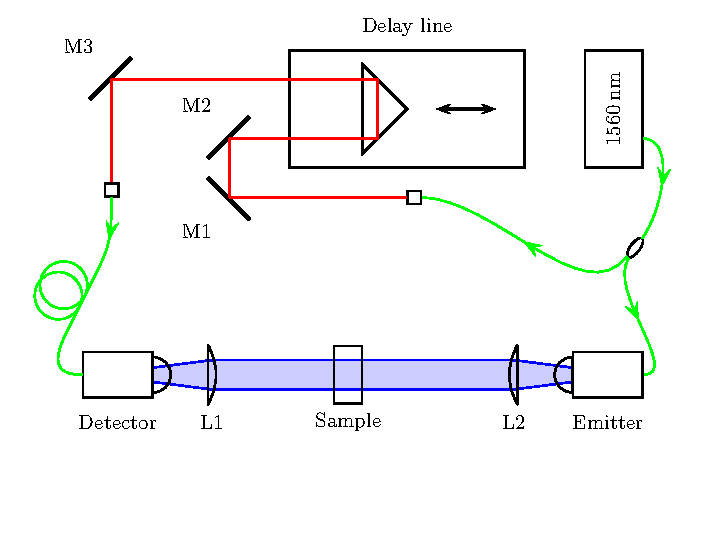
\includegraphics[scale=0.65]{images/TDS/Setup-THz-TDS-SimpleExample.pdf}
    \caption{Example of a general THz-TDS setup in transmission geometry employing PCAs as detector and emitter. The laser pulses are guided using mirrors M1-M3. Two polyethylene lenses (L1, L2) are used to collimate the THz radiation and focus it on the detector module.}
    \label{fig:Setup-THz-TDS-SimpleExample}
\end{figure}

Additional examples of THz-TDS spectrometers are presented in chapter \ref{ch:setups} which utilize the emission and detection scheme described in this chapter. These two setups were used for a part of the measurements performed in this work. In the following chapter we introduce the fundamentals of EM wave polarization including different mathematical (and graphical) representations of the polarization state as well as the propagation of light in anisotropic media.